\documentclass[handout, noauthor, nooutcomes]{ximera}


\graphicspath{
  {./}
  {1-1QuantitativeReasoning/}
  {1-2RelationsAndGraphs/}
  {1-3ChangingInTandem/}
  {2-1LinearEquations/}
  {2-2LinearModeling/}
  {2-3ExponentialModeling/}
  {3-1WhatIsAFunction/}
  {3-2FunctionProperties/}
  {3-3AverageRatesOfChange/}
  {4-1BuildingNewFunctions/}
  {4-2Polynomials/}
  {5-1RationalFunctions/}
   {5-2ExponentialFunctions/}
  {6-1Domain/}
  {6-2Range/}
  {6-3CompositionOfFunctions/}
  {7-1ZerosOfFunctions/}
  {7-XZerosOfPolynomials/}
  {7-2ZerosOfFamousFunctions/}
  {8-0Review/}
  {8-1FunctionTransformations/}
  {8-2SolvingInequalities/}
  {8-3FunctionTransformationsProject/}
  {9-1RightTriangleTrig/}
  {9-2TheUnitCircle/}
  {9-3TrigIdentities/}
  {10-1UnitCircleToFunctionGraph/}
  {10-2TrigFunctions/}
  {10-3SomeApplicationsOfTrig/}
  {11-1InverseFunctionsRevisited/}
  {11-2Logarithms/}
  {11-3InverseTrig/}
  {12-1SystemsOfEquations/}
  {12-2NonlinearSystems/}
  {12-3ApplicationsOfSystems/}
  {13-1SecantLinesRevisited/}
  {13-2Functions-TheBigPicture/}
  {14-1DisplacementVsDistance/}
  {1-1QuantitativeReasoning/exercises/}
  {1-2RelationsAndGraphs/exercises/}
  {../1-3ChangingInTandem/exercises/}
  {../2-1LinearEquations/exercises/}
  {../2-2LinearModeling/exercises/}
  {../2-3ExponentialModeling/exercises/}
  {../3-1WhatIsAFunction/exercises/}
  {../3-2FunctionProperties/exercises/}
  {../3-3AverageRatesOfChange/exercises/}
  {../5-2ExponentialFunctions/exercises/}
  {../4-1BuildingNewFunctions/exercises/}
  {../4-2Polynomials/exercises/}
  {../5-1RationalFunctions/exercises/}
  {../6-1Domain/exercises/}
  {../6-2Range/exercises/}
  {../6-3CompositionOfFunctions/exercises/}
  {../7-1ZerosOfFunctions/exercises/}
  {../7-XZerosOfPolynomials/exercises/}
  {../7-2ZerosOfFamousFunctions/exercises/}
  {../8-1FunctionTransformations/exercises/}
  {../12-1SystemsOfEquations/exercises/}
  {../8-3FunctionTransformationsProject/exercises/}
  {../8-0Review/exercises/}
  {../8-2SolvingInequalities/exercises/}
  {../8-3FunctionTransformationsProject/exercises/}
  {../9-1RightTriangleTrig/exercises/}
  {../9-2TheUnitCircle/exercises/}
  {../9-3TrigIdentities/exercises/}
  {../10-1UnitCircleToFunctionGraph/exercises/}
  {../10-2TrigFunctions/exercises/}
  {../10-3SomeApplicationsOfTrig/exercises/}
  {../11-1InverseFunctionsRevisited/exercises/}
  {../11-2Logarithms/exercises/}
  {../11-3InverseTrig/exercises/}
  {../12-1SystemsOfEquations/exercises/}
  {../12-2NonlinearSystems/exercises/}
  {../12-3ApplicationsOfSystems/exercises/}
  {../13-1SecantLinesRevisited/exercises/}
  {../13-2Functions-TheBigPicture/exercises/}
  {../14-1DisplacementVsDistance/exercises/}
}

\DeclareGraphicsExtensions{.pdf,.png,.jpg,.eps}

\newcommand{\mooculus}{\textsf{\textbf{MOOC}\textnormal{\textsf{ULUS}}}}

\usepackage[makeroom]{cancel} %% for strike outs

\ifxake
\else
\usepackage[most]{tcolorbox}
\fi


%\typeout{************************************************}
%\typeout{New Environments}
%\typeout{************************************************}

%% to fix for web can be removed when deployed offically with ximera2
\let\image\relax\let\endimage\relax
\NewEnviron{image}{% 
  \begin{center}\BODY\end{center}% center
}



\NewEnviron{folder}{
      \addcontentsline{toc}{section}{\textbf{\BODY}}
}

\ifxake
\let\summary\relax
\let\endsummary\relax
\newtheorem*{summary}{Summary}
\newtheorem*{callout}{Callout}
\newtheorem*{overview}{Overview}
\newtheorem*{objectives}{Objectives}
\newtheorem*{motivatingQuestions}{Motivating Questions}
\newtheorem*{MM}{Metacognitive Moment}
      
%% NEEDED FOR XIMERA 2
%\ximerizedEnvironment{summary}
%\ximerizedEnvironment{callout}
%\ximerizedEnvironment{overview} 
%\ximerizedEnvironment{objectives}
%\ximerizedEnvironment{motivatingQuestions}
%\ximerizedEnvironment{MM}
\else
%% CALLOUT
\NewEnviron{callout}{
  \begin{tcolorbox}[colback=blue!5, breakable,pad at break*=1mm]
      \BODY
  \end{tcolorbox}
}
%% MOTIVATING QUESTIONS
\NewEnviron{motivatingQuestions}{
  \begin{tcolorbox}[ breakable,pad at break*=1mm]
    \textbf{\Large Motivating Questions}\hfill
    %\begin{itemize}[label=\textbullet]
      \BODY
    %\end{itemize}
  \end{tcolorbox}
}
%% OBJECTIVES
\NewEnviron{objectives}{  
    \vspace{.5in}
      %\begin{tcolorbox}[colback=orange!5, breakable,pad at break*=1mm]
    \textbf{\Large Learning Objectives}
    \begin{itemize}[label=\textbullet]
      \BODY
    \end{itemize}
    %\end{tcolorbox}
}
%% DEFINITION
\let\definition\relax
\let\enddefinition\relax
\NewEnviron{definition}{
  \begin{tcolorbox}[ breakable,pad at break*=1mm]
    \noindent\textbf{Definition}~
      \BODY
  \end{tcolorbox}
}
%% OVERVIEW
\let\overview\relax
\let\overview\relax
\NewEnviron{overview}{
  \begin{tcolorbox}[ breakable,pad at break*=1mm]
    \textbf{\Large Overview}
    %\begin{itemize}[label=\textbullet] %% breaks Xake
      \BODY
    %\end{itemize}
  \end{tcolorbox}
}
%% SUMMARY
\let\summary\relax
\let\endsummary\relax
\NewEnviron{summary}{
  \begin{tcolorbox}[ breakable,pad at break*=1mm]
    \textbf{\Large Summary}
    %\begin{itemize}[label=\textbullet] %% breaks Xake
      \BODY
    %\end{itemize}
  \end{tcolorbox}
}
%% REMARK
\let\remark\relax
\let\endremark\relax
\NewEnviron{remark}{
  \begin{tcolorbox}[colback=green!5, breakable,pad at break*=1mm]
    \noindent\textbf{Remark}~
      \BODY
  \end{tcolorbox}
}
%% EXPLANATION
\let\explanation\relax
\let\endexplanation\relax
\NewEnviron{explanation}{
    \normalfont
    \noindent\textbf{Explanation}~
      \BODY
}
%% EXPLORATION
\let\exploration\relax
\let\endexploration\relax
\NewEnviron{exploration}{
  \begin{tcolorbox}[colback=yellow!10, breakable,pad at break*=1mm]
    \noindent\textbf{Exploration}~
      \BODY
  \end{tcolorbox}
}
%% METACOGNITIVE MOMENTS
\let\MM\relax
\let\endMM\relax
\NewEnviron{MM}{
  \begin{tcolorbox}[colback=pink!15, breakable,pad at break*=1mm]
    \noindent\textbf{Metacognitive Moment}~
      \BODY
  \end{tcolorbox}
}


\fi





%Notes on what envirnoment to use:  Example with Explanation in text; if they are supposed to answer- Problem; no answer - Exploration


%\typeout{************************************************}
%% Header and footers
%\typeout{************************************************}

\newcommand{\licenseAcknowledgement}{Licensed under Creative Commons 4.0}
\newcommand{\licenseAPC}{\renewcommand{\licenseAcknowledgement}{\textbf{Acknowledgements:} Active Prelude to Calculus (https://activecalculus.org/prelude) }}
\newcommand{\licenseSZ}{\renewcommand{\licenseAcknowledgement}{\textbf{Acknowledgements:} Stitz Zeager Open Source Mathematics (https://www.stitz-zeager.com/) }}
\newcommand{\licenseAPCSZ}{\renewcommand{\licenseAcknowledgement}{\textbf{Acknowledgements:} Active Prelude to Calculus (https://activecalculus.org/prelude) and Stitz Zeager Open Source Mathematics (https://www.stitz-zeager.com/) }}
\newcommand{\licenseORCCA}{\renewcommand{\licenseAcknowledgement}{\textbf{Acknowledgements:}Original source material, products with readable and accessible
math content, and other information freely available at pcc.edu/orcca.}}
\newcommand{\licenseY}{\renewcommand{\licenseAcknowledgement}{\textbf{Acknowledgements:} Yoshiwara Books (https://yoshiwarabooks.org/)}}
\newcommand{\licenseOS}{\renewcommand{\licenseAcknowledgement}{\textbf{Acknowledgements:} OpenStax College Algebra (https://openstax.org/details/books/college-algebra)}}
\newcommand{\licenseAPCSZCSCC}{\renewcommand{\licenseAcknowledgement}{\textbf{Acknowledgements:} Active Prelude to Calculus (https://activecalculus.org/prelude), Stitz Zeager Open Source Mathematics (https://www.stitz-zeager.com/), CSCC PreCalculus and Calculus texts (https://ximera.osu.edu/csccmathematics)}}

\ifxake\else %% do nothing on the website
\usepackage{fancyhdr}
\pagestyle{fancy}
\fancyhf{}
\fancyhead[R]{\sectionmark}
\fancyfoot[L]{\thepage}
\fancyfoot[C]{\licenseAcknowledgement}
\renewcommand{\headrulewidth}{0pt}
\renewcommand{\footrulewidth}{0pt}
\fi

%%%%%%%%%%%%%%%%



%\typeout{************************************************}
%\typeout{Table of Contents}
%\typeout{************************************************}


%% Edit this to change the font style
\newcommand{\sectionHeadStyle}{\sffamily\bfseries}


\makeatletter

%% part uses arabic numerals
\renewcommand*\thepart{\arabic{part}}


\ifxake\else
\renewcommand\chapterstyle{%
  \def\maketitle{%
    \addtocounter{titlenumber}{1}%
    \pagestyle{fancy}
    \phantomsection
    \addcontentsline{toc}{section}{\textbf{\thepart.\thetitlenumber\hspace{1em}\@title}}%
                    {\flushleft\small\sectionHeadStyle\@pretitle\par\vspace{-1.5em}}%
                    {\flushleft\LARGE\sectionHeadStyle\thepart.\thetitlenumber\hspace{1em}\@title \par }%
                    {\setcounter{problem}{0}\setcounter{sectiontitlenumber}{0}}%
                    \par}}





\renewcommand\sectionstyle{%
  \def\maketitle{%
    \addtocounter{sectiontitlenumber}{1}
    \pagestyle{fancy}
    \phantomsection
    \addcontentsline{toc}{subsection}{\thepart.\thetitlenumber.\thesectiontitlenumber\hspace{1em}\@title}%
    {\flushleft\small\sectionHeadStyle\@pretitle\par\vspace{-1.5em}}%
    {\flushleft\Large\sectionHeadStyle\thepart.\thetitlenumber.\thesectiontitlenumber\hspace{1em}\@title \par}%
    %{\setcounter{subsectiontitlenumber}{0}}%
    \par}}



\renewcommand\section{\@startsection{paragraph}{10}{\z@}%
                                     {-3.25ex\@plus -1ex \@minus -.2ex}%
                                     {1.5ex \@plus .2ex}%
                                     {\normalfont\large\sectionHeadStyle}}
\renewcommand\subsection{\@startsection{subparagraph}{10}{\z@}%
                                    {3.25ex \@plus1ex \@minus.2ex}%
                                    {-1em}%
                                    {\normalfont\normalsize\sectionHeadStyle}}

\fi

%% redefine Part
\renewcommand\part{%
   {\setcounter{titlenumber}{0}}
  \if@openright
    \cleardoublepage
  \else
    \clearpage
  \fi
  \thispagestyle{plain}%
  \if@twocolumn
    \onecolumn
    \@tempswatrue
  \else
    \@tempswafalse
  \fi
  \null\vfil
  \secdef\@part\@spart}

\def\@part[#1]#2{%
    \ifnum \c@secnumdepth >-2\relax
      \refstepcounter{part}%
      \addcontentsline{toc}{part}{\thepart\hspace{1em}#1}%
    \else
      \addcontentsline{toc}{part}{#1}%
    \fi
    \markboth{}{}%
    {\centering
     \interlinepenalty \@M
     \normalfont
     \ifnum \c@secnumdepth >-2\relax
       \huge\sffamily\bfseries \partname\nobreakspace\thepart
       \par
       \vskip 20\p@
     \fi
     \Huge \bfseries #2\par}%
    \@endpart}
\def\@spart#1{%
    {\centering
     \interlinepenalty \@M
     \normalfont
     \Huge \bfseries #1\par}%
    \@endpart}
\def\@endpart{\vfil\newpage
              \if@twoside
               \if@openright
                \null
                \thispagestyle{empty}%
                \newpage
               \fi
              \fi
              \if@tempswa
                \twocolumn
                \fi}



\makeatother





%\typeout{************************************************}
%\typeout{Stuff from Ximera}
%\typeout{************************************************}



\usepackage{array}  %% This is for typesetting long division
\setlength{\extrarowheight}{+.1cm}
\newdimen\digitwidth
\settowidth\digitwidth{9}
\def\divrule#1#2{
\noalign{\moveright#1\digitwidth
\vbox{\hrule width#2\digitwidth}}}





\newcommand{\RR}{\mathbb R}
\newcommand{\R}{\mathbb R}
\newcommand{\N}{\mathbb N}
\newcommand{\Z}{\mathbb Z}

\newcommand{\sagemath}{\textsf{SageMath}}


\def\d{\,d}
%\renewcommand{\d}{\mathop{}\!d}
\newcommand{\dd}[2][]{\frac{\d #1}{\d #2}}
\newcommand{\pp}[2][]{\frac{\partial #1}{\partial #2}}
\renewcommand{\l}{\ell}
\newcommand{\ddx}{\frac{d}{\d x}}



%\newcommand{\unit}{\,\mathrm}
\newcommand{\unit}{\mathop{}\!\mathrm}
\newcommand{\eval}[1]{\bigg[ #1 \bigg]}
\newcommand{\seq}[1]{\left( #1 \right)}
\renewcommand{\epsilon}{\varepsilon}
\renewcommand{\phi}{\varphi}


\renewcommand{\iff}{\Leftrightarrow}

\DeclareMathOperator{\arccot}{arccot}
\DeclareMathOperator{\arcsec}{arcsec}
\DeclareMathOperator{\arccsc}{arccsc}
\DeclareMathOperator{\sign}{sign}


%\DeclareMathOperator{\divergence}{divergence}
%\DeclareMathOperator{\curl}[1]{\grad\cross #1}
\newcommand{\lto}{\mathop{\longrightarrow\,}\limits}

\renewcommand{\bar}{\overline}

\colorlet{textColor}{black}
\colorlet{background}{white}
\colorlet{penColor}{blue!50!black} % Color of a curve in a plot
\colorlet{penColor2}{red!50!black}% Color of a curve in a plot
\colorlet{penColor3}{red!50!blue} % Color of a curve in a plot
\colorlet{penColor4}{green!50!black} % Color of a curve in a plot
\colorlet{penColor5}{orange!80!black} % Color of a curve in a plot
\colorlet{penColor6}{yellow!70!black} % Color of a curve in a plot
\colorlet{fill1}{penColor!20} % Color of fill in a plot
\colorlet{fill2}{penColor2!20} % Color of fill in a plot
\colorlet{fillp}{fill1} % Color of positive area
\colorlet{filln}{penColor2!20} % Color of negative area
\colorlet{fill3}{penColor3!20} % Fill
\colorlet{fill4}{penColor4!20} % Fill
\colorlet{fill5}{penColor5!20} % Fill
\colorlet{gridColor}{gray!50} % Color of grid in a plot

\newcommand{\surfaceColor}{violet}
\newcommand{\surfaceColorTwo}{redyellow}
\newcommand{\sliceColor}{greenyellow}




\pgfmathdeclarefunction{gauss}{2}{% gives gaussian
  \pgfmathparse{1/(#2*sqrt(2*pi))*exp(-((x-#1)^2)/(2*#2^2))}%
}





%\typeout{************************************************}
%\typeout{ORCCA Preamble.Tex}
%\typeout{************************************************}


%% \usepackage{geometry}
%% \geometry{letterpaper,total={408pt,9.0in}}
%% Custom Page Layout Adjustments (use latex.geometry)
%% \usepackage{amsmath,amssymb}
%% \usepackage{pgfplots}
\usepackage{pifont}                                         %needed for symbols, s.a. airplane symbol
\usetikzlibrary{positioning,fit,backgrounds}                %needed for nested diagrams
\usetikzlibrary{calc,trees,positioning,arrows,fit,shapes}   %needed for set diagrams
\usetikzlibrary{decorations.text}                           %needed for text following a curve
\usetikzlibrary{arrows,arrows.meta}                         %needed for open/closed intervals
\usetikzlibrary{positioning,3d,shapes.geometric}            %needed for 3d number sets tower

%% NEEDED FOR XIMERA 1
%\usetkzobj{all}       %NO LONGER VALID
%%%%%%%%%%%%%%

\usepackage{tikz-3dplot}
\usepackage{tkz-euclide}                     %needed for triangle diagrams
\usepgfplotslibrary{fillbetween}                            %shade regions of a plot
\usetikzlibrary{shadows}                                    %function diagrams
\usetikzlibrary{positioning}                                %function diagrams
\usetikzlibrary{shapes}                                     %function diagrams
%%% global colors from https://www.pcc.edu/web-services/style-guide/basics/color/ %%%
\definecolor{ruby}{HTML}{9E0C0F}
\definecolor{turquoise}{HTML}{008099}
\definecolor{emerald}{HTML}{1c8464}
\definecolor{amber}{HTML}{c7502a}
\definecolor{amethyst}{HTML}{70485b}
\definecolor{sapphire}{HTML}{263c53}
\colorlet{firstcolor}{sapphire}
\colorlet{secondcolor}{turquoise}
\colorlet{thirdcolor}{emerald}
\colorlet{fourthcolor}{amber}
\colorlet{fifthcolor}{amethyst}
\colorlet{sixthcolor}{ruby}
\colorlet{highlightcolor}{green!50!black}
\colorlet{graphbackground}{white}
\colorlet{wood}{brown!60!white}
%%% curve, dot, and graph custom styles %%%
\pgfplotsset{firstcurve/.style      = {color=firstcolor,  mark=none, line width=1pt, {Kite}-{Kite}, solid}}
\pgfplotsset{secondcurve/.style     = {color=secondcolor, mark=none, line width=1pt, {Kite}-{Kite}, solid}}
\pgfplotsset{thirdcurve/.style      = {color=thirdcolor,  mark=none, line width=1pt, {Kite}-{Kite}, solid}}
\pgfplotsset{fourthcurve/.style     = {color=fourthcolor, mark=none, line width=1pt, {Kite}-{Kite}, solid}}
\pgfplotsset{fifthcurve/.style      = {color=fifthcolor,  mark=none, line width=1pt, {Kite}-{Kite}, solid}}
\pgfplotsset{highlightcurve/.style  = {color=highlightcolor,  mark=none, line width=5pt, -, opacity=0.3}}   % thick, opaque curve for highlighting
\pgfplotsset{asymptote/.style       = {color=gray, mark=none, line width=1pt, <->, dashed}}
\pgfplotsset{symmetryaxis/.style    = {color=gray, mark=none, line width=1pt, <->, dashed}}
\pgfplotsset{guideline/.style       = {color=gray, mark=none, line width=1pt, -}}
\tikzset{guideline/.style           = {color=gray, mark=none, line width=1pt, -}}
\pgfplotsset{altitude/.style        = {dashed, color=gray, thick, mark=none, -}}
\tikzset{altitude/.style            = {dashed, color=gray, thick, mark=none, -}}
\pgfplotsset{radius/.style          = {dashed, thick, mark=none, -}}
\tikzset{radius/.style              = {dashed, thick, mark=none, -}}
\pgfplotsset{rightangle/.style      = {color=gray, mark=none, -}}
\tikzset{rightangle/.style          = {color=gray, mark=none, -}}
\pgfplotsset{closedboundary/.style  = {color=black, mark=none, line width=1pt, {Kite}-{Kite},solid}}
\tikzset{closedboundary/.style      = {color=black, mark=none, line width=1pt, {Kite}-{Kite},solid}}
\pgfplotsset{openboundary/.style    = {color=black, mark=none, line width=1pt, {Kite}-{Kite},dashed}}
\tikzset{openboundary/.style        = {color=black, mark=none, line width=1pt, {Kite}-{Kite},dashed}}
\tikzset{verticallinetest/.style    = {color=gray, mark=none, line width=1pt, <->,dashed}}
\pgfplotsset{soliddot/.style        = {color=firstcolor,  mark=*, only marks}}
\pgfplotsset{hollowdot/.style       = {color=firstcolor,  mark=*, only marks, fill=graphbackground}}
\pgfplotsset{blankgraph/.style      = {xmin=-10, xmax=10,
                                        ymin=-10, ymax=10,
                                        axis line style={-, draw opacity=0 },
                                        axis lines=box,
                                        major tick length=0mm,
                                        xtick={-10,-9,...,10},
                                        ytick={-10,-9,...,10},
                                        grid=major,
                                        grid style={solid,gray!20},
                                        xticklabels={,,},
                                        yticklabels={,,},
                                        minor xtick=,
                                        minor ytick=,
                                        xlabel={},ylabel={},
                                        width=0.75\textwidth,
                                      }
            }
\pgfplotsset{numberline/.style      = {xmin=-10,xmax=10,
                                        minor xtick={-11,-10,...,11},
                                        xtick={-10,-5,...,10},
                                        every tick/.append style={thick},
                                        axis y line=none,
                                        y=15pt,
                                        axis lines=middle,
                                        enlarge x limits,
                                        grid=none,
                                        clip=false,
                                        axis background/.style={},
                                        after end axis/.code={
                                          \path (axis cs:0,0)
                                          node [anchor=north,yshift=-0.075cm] {\footnotesize 0};
                                        },
                                        every axis x label/.style={at={(current axis.right of origin)},anchor=north},
                                      }
            }
\pgfplotsset{openinterval/.style={color=firstcolor,mark=none,ultra thick,{Parenthesis}-{Parenthesis}}}
\pgfplotsset{openclosedinterval/.style={color=firstcolor,mark=none,ultra thick,{Parenthesis}-{Bracket}}}
\pgfplotsset{closedinterval/.style={color=firstcolor,mark=none,ultra thick,{Bracket}-{Bracket}}}
\pgfplotsset{closedopeninterval/.style={color=firstcolor,mark=none,ultra thick,{Bracket}-{Parenthesis}}}
\pgfplotsset{infiniteopeninterval/.style={color=firstcolor,mark=none,ultra thick,{Kite}-{Parenthesis}}}
\pgfplotsset{openinfiniteinterval/.style={color=firstcolor,mark=none,ultra thick,{Parenthesis}-{Kite}}}
\pgfplotsset{infiniteclosedinterval/.style={color=firstcolor,mark=none,ultra thick,{Kite}-{Bracket}}}
\pgfplotsset{closedinfiniteinterval/.style={color=firstcolor,mark=none,ultra thick,{Bracket}-{Kite}}}
\pgfplotsset{infiniteinterval/.style={color=firstcolor,mark=none,ultra thick,{Kite}-{Kite}}}
\pgfplotsset{interval/.style= {ultra thick, -}}
%%% cycle list of plot styles for graphs with multiple plots %%%
\pgfplotscreateplotcyclelist{pccstylelist}{%
  firstcurve\\%
  secondcurve\\%
  thirdcurve\\%
  fourthcurve\\%
  fifthcurve\\%
}
%%% default plot settings %%%
\pgfplotsset{every axis/.append style={
  axis x line=middle,    % put the x axis in the middle
  axis y line=middle,    % put the y axis in the middle
  axis line style={<->}, % arrows on the axis
  scaled ticks=false,
  tick label style={/pgf/number format/fixed},
  xlabel={$x$},          % default put x on x-axis
  ylabel={$y$},          % default put y on y-axis
  xmin = -7,xmax = 7,    % most graphs have this window
  ymin = -7,ymax = 7,    % most graphs have this window
  domain = -7:7,
  xtick = {-6,-4,...,6}, % label these ticks
  ytick = {-6,-4,...,6}, % label these ticks
  yticklabel style={inner sep=0.333ex},
  minor xtick = {-7,-6,...,7}, % include these ticks, some without label
  minor ytick = {-7,-6,...,7}, % include these ticks, some without label
  scale only axis,       % don't consider axis and tick labels for width and height calculation
  cycle list name=pccstylelist,
  tick label style={font=\footnotesize},
  legend cell align=left,
  grid = both,
  grid style = {solid,gray!20},
  axis background/.style={fill=graphbackground},
}}
\pgfplotsset{framed/.style={axis background/.style ={draw=gray}}}
%\pgfplotsset{framed/.style={axis background/.style ={draw=gray,fill=graphbackground,rounded corners=3ex}}}
%%% other tikz (not pgfplots) settings %%%
%\tikzset{axisnode/.style={font=\scriptsize,text=black}}
\tikzset{>=stealth}
%%% for nested diagram in types of numbers section %%%
\newcommand\drawnestedsets[4]{
  \def\position{#1}             % initial position
  \def\nbsets{#2}               % number of sets
  \def\listofnestedsets{#3}     % list of sets
  \def\reversedlistofcolors{#4} % reversed list of colors
  % position and draw labels of sets
  \coordinate (circle-0) at (#1);
  \coordinate (set-0) at (#1);
  \foreach \set [count=\c] in \listofnestedsets {
    \pgfmathtruncatemacro{\cminusone}{\c - 1}
    % label of current set (below previous nested set)
    \node[below=3pt of circle-\cminusone,inner sep=0]
    (set-\c) {\set};
    % current set (fit current label and previous set)
    \node[circle,inner sep=0,fit=(circle-\cminusone)(set-\c)]
    (circle-\c) {};
  }
  % draw and fill sets in reverse order
  \begin{scope}[on background layer]
    \foreach \col[count=\c] in \reversedlistofcolors {
      \pgfmathtruncatemacro{\invc}{\nbsets-\c}
      \pgfmathtruncatemacro{\invcplusone}{\invc+1}
      \node[circle,draw,fill=\col,inner sep=0,
      fit=(circle-\invc)(set-\invcplusone)] {};
    }
  \end{scope}
  }
\ifdefined\tikzset
\tikzset{ampersand replacement = \amp}
\fi
\newcommand{\abs}[1]{\left\lvert#1\right\rvert}
%\newcommand{\point}[2]{\left(#1,#2\right)}
\newcommand{\highlight}[1]{\definecolor{sapphire}{RGB}{59,90,125} {\color{sapphire}{{#1}}}}
\newcommand{\firsthighlight}[1]{\definecolor{sapphire}{RGB}{59,90,125} {\color{sapphire}{{#1}}}}
\newcommand{\secondhighlight}[1]{\definecolor{emerald}{RGB}{20,97,75} {\color{emerald}{{#1}}}}
\newcommand{\unhighlight}[1]{{\color{black}{{#1}}}}
\newcommand{\lowlight}[1]{{\color{lightgray}{#1}}}
\newcommand{\attention}[1]{\mathord{\overset{\downarrow}{#1}}}
\newcommand{\nextoperation}[1]{\mathord{\boxed{#1}}}
\newcommand{\substitute}[1]{{\color{blue}{{#1}}}}
\newcommand{\pinover}[2]{\overset{\overset{\mathrm{\ #2\ }}{|}}{\strut #1 \strut}}
\newcommand{\addright}[1]{{\color{blue}{{{}+#1}}}}
\newcommand{\addleft}[1]{{\color{blue}{{#1+{}}}}}
\newcommand{\subtractright}[1]{{\color{blue}{{{}-#1}}}}
\newcommand{\multiplyright}[2][\cdot]{{\color{blue}{{{}#1#2}}}}
\newcommand{\multiplyleft}[2][\cdot]{{\color{blue}{{#2#1{}}}}}
\newcommand{\divideunder}[2]{\frac{#1}{{\color{blue}{{#2}}}}}
\newcommand{\divideright}[1]{{\color{blue}{{{}\div#1}}}}
\newcommand{\negate}[1]{{\color{blue}{{-}}}\left(#1\right)}
\newcommand{\cancelhighlight}[1]{\definecolor{sapphire}{RGB}{59,90,125}{\color{sapphire}{{\cancel{#1}}}}}
\newcommand{\secondcancelhighlight}[1]{\definecolor{emerald}{RGB}{20,97,75}{\color{emerald}{{\bcancel{#1}}}}}
\newcommand{\thirdcancelhighlight}[1]{\definecolor{amethyst}{HTML}{70485b}{\color{amethyst}{{\xcancel{#1}}}}}
\newcommand{\lt}{<} %% Bart: WHY?
\newcommand{\gt}{>} %% Bart: WHY?
\newcommand{\amp}{&} %% Bart: WHY?


%%% These commands break Xake
%% \newcommand{\apple}{\text{🍎}}
%% \newcommand{\banana}{\text{🍌}}
%% \newcommand{\pear}{\text{🍐}}
%% \newcommand{\cat}{\text{🐱}}
%% \newcommand{\dog}{\text{🐶}}

\newcommand{\apple}{PICTURE OF APPLE}
\newcommand{\banana}{PICTURE OF BANANA}
\newcommand{\pear}{PICTURE OF PEAR}
\newcommand{\cat}{PICTURE OF CAT}
\newcommand{\dog}{PICTURE OF DOG}


%%%%% INDEX STUFF
\newcommand{\dfn}[1]{\textbf{#1}\index{#1}}
\usepackage{imakeidx}
\makeindex[intoc]
\makeatletter
\gdef\ttl@savemark{\sectionmark{}}
\makeatother












 % for drawing cube in Optimization problem
\usetikzlibrary{quotes,arrows.meta}
\tikzset{
  annotated cuboid/.pic={
    \tikzset{%
      every edge quotes/.append style={midway, auto},
      /cuboid/.cd,
      #1
    }
    \draw [every edge/.append style={pic actions, densely dashed, opacity=.5}, pic actions]
    (0,0,0) coordinate (o) -- ++(-\cubescale*\cubex,0,0) coordinate (a) -- ++(0,-\cubescale*\cubey,0) coordinate (b) edge coordinate [pos=1] (g) ++(0,0,-\cubescale*\cubez)  -- ++(\cubescale*\cubex,0,0) coordinate (c) -- cycle
    (o) -- ++(0,0,-\cubescale*\cubez) coordinate (d) -- ++(0,-\cubescale*\cubey,0) coordinate (e) edge (g) -- (c) -- cycle
    (o) -- (a) -- ++(0,0,-\cubescale*\cubez) coordinate (f) edge (g) -- (d) -- cycle;
    \path [every edge/.append style={pic actions, |-|}]
    (b) +(0,-5pt) coordinate (b1) edge ["x"'] (b1 -| c)
    (b) +(-5pt,0) coordinate (b2) edge ["y"] (b2 |- a)
    (c) +(3.5pt,-3.5pt) coordinate (c2) edge ["x"'] ([xshift=3.5pt,yshift=-3.5pt]e)
    ;
  },
  /cuboid/.search also={/tikz},
  /cuboid/.cd,
  width/.store in=\cubex,
  height/.store in=\cubey,
  depth/.store in=\cubez,
  units/.store in=\cubeunits,
  scale/.store in=\cubescale,
  width=10,
  height=10,
  depth=10,
  units=cm,
  scale=.1,
}

\author{}
\license{Creative Commons Attribution-ShareAlike 4.0 International License}
\acknowledgement{}

\title{Reflections of Functions}

\begin{document}
\begin{abstract}
  
\end{abstract}
\maketitle


%%\typeout{************************************************}
%%\typeout{Motivating Questions}
%%\typeout{************************************************}
%
%\begin{motivatingQuestions}\begin{itemize}
%\item 
%\item 
%\item 
%\end{itemize}\end{motivatingQuestions}


%\typeout{************************************************}
%\typeout{Reflections Across Axes}
%\typeout{************************************************}

%\section{Reflections Across Axes}
%Points $(x,y)$ and $(x,-y)$ are reflections of each other across the x-axis. Points $(x, y)$ and $(-x, y)$ are reflections of each other across the y-axis. In general, two points that are symmetric with respect to a line are reflections of each other across that line.
%\begin{image}
%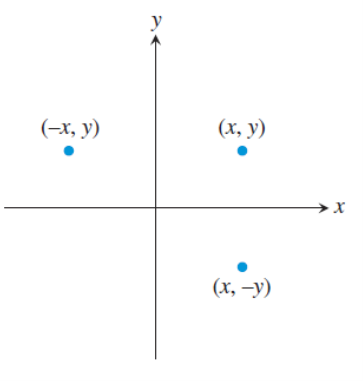
\includegraphics[]{images/reflectiongraph}
%\end{image}
%\begin{callout}
%The following transformations result in reflections of the graph of $y = f(x)$
%\begin{itemize}
%\item Reflection across the x-axis
%\[
%y=-f(x)
%\]
%\item Reflection across the y-axis
%\[
%y=f(-x)
%\]
%\item Reflection through the origin
%\[
%y=-f(-x)
%\]
%\end{itemize}
%\end{callout}
%\begin{example}
%Find an equation for the reflection of $f(x) = \frac{5x - 9}{x^2+3}$ across each axis.
%\\
%\begin{explanation}
%Across the x-axis: $y = -f(x) = -\frac{5x-9}{x^2+3}=\frac{9-5x}{x^2+3}$
%\\
%Across the y-axis: $y = f(-x) = \frac{5(-x)-9}{(-x)^2+3}=\frac{-5x-9}{x^2+3}$
%\end{explanation}
%\end{example}

%\typeout{************************************************}
%\typeout{Putting it Together}
%\typeout{************************************************}

\section{Introduction}
In this section, we will review our earlier discussion about function transformations. In addition, we'll explore what happens when multiple function transformations occur. 

\section{Review of Single Transformations}
The following table gives the formulas and descriptions of all the function transformations we learned about. If $f$ is the parent function, then the formula in the left column gives the function that corresponds to the transformation of the graph given in the middle column. The right column gives the new location of the point $(x, y)$ on the graph of $f$. 
$$
\begin{array}{c|c|c}
\text{Formula} & \text{Description} & \text{Transformed Point}\\
\hline
f(x) + k & \text{shift up }k\text{, for } k > 0 &(x, y + k) \\
f(x) - k & \text{shift down }k\text{, for } k > 0& (x, y - k)\\
af(x) & \text{vertical stretch by }a\text{, for }a > 1 & (x, ay)\\
\frac{1}{a}f(x) & \text{vertical compression by }a\text{, for }a > 1 & \left(x, \frac{y}{a}\right)\\
f(x - h) & \text{shift right by }h\text{, for }h > 0 & (x + h, y)\\
f(x + h) & \text{shift left by }h\text{, for }h > 0 & (x - h, y)\\
f(bx) & \text{horizontal compression by }b\text{, for }b > 1 & \left(\frac{x}{b}, y \right)\\
f\left(\frac{x}{b}\right) & \text{horizontal stretch by }a\text{, for }b > 1 & (bx, y)\\
-f(x) & \text{vertical flip (flip over }x\text{-axis)} & (x, -y)\\
f(-x) & \text{horizontal flip (flip over }y\text{-axis)} & (-x, y)\\
-f(-x) & \text{180}^\circ\text{ rotation (flip over }x\text{-axis and }x\text{-axis)} & (-x, -y)\\
\end{array}
$$

\section{Putting it Together}
Transformations may be performed one after another. If the transformations include stretches, shrinks, or reflections, the order in which the transformations are performed may make a difference. In those cases, be sure to pay particular attention to the order.

\begin{example}
\begin{enumerate}
\item The graph of $y=x^2$ undergoes the following transformations, in order. Find the equation of the graph that results.
\begin{itemize}
\item a horizontal shift 2 units to the right
\item a vertical stretch by a factor of 3
\item a vertical shift 5 units up
\end{itemize}
\item Apply the transformations above in the opposite order and find the equation of the graph that results.
\end{enumerate}
\begin{explanation}
\begin{enumerate}
\item Applying the transformations in order we have\\
$
\begin{array}{lc}
y = x^2& \text{Parent function}\\
y = (x-2)^2& \text{Horizontal shift} \\
y = 3(x-2)^2& \text{Vertical stretch} \\
y = 3(x-2)^2+5& \text{Vertical shift}\\
y = 3x^2 - 12x + 17& \text{Expanded form}
\end{array}
$
\item Applying the transformations in the opposite order we have\\
$
\begin{array}{lc}
y = x^2& \text{Parent function}\\
y = x^2 + 5 & \text{Vertical shift} \\
y = 3(x^2+5)& \text{Vertical stretch} \\
y = 3((x-2)^2+5) & \text{Horizontal shift}\\
y = 3x^2 - 12x + 27& \text{Expanded form}
\end{array}
$
\end{enumerate}
This shows that changing the order in which the transformations are applied may end up changing the resulting function. 
\end{explanation}
\end{example}

The previous example shows how to construct the formula of a function given a sequence of transformations. One might wonder how to find the transformations applied to a parent function's graph given a complicated formula. That is, if we know a formula $af(bx + h) + k$, can we reconstruct the sequence of transformations? There are two parts to this: finding the transformations and finding the order of those transformations. The following example gives some of the reasoning behind the process. 

\begin{example}
Given a function $f$ defined by $f(x) = 3|2x + 7| - 2$, find its parent function and list the transformations, in order, applied to the parent function's graph to produce the graph of $f$. 
\begin{explanation}
The parent function $f_0$ is given by $f_0(x) = |x|$. We will use subscripts to denote the intermediate steps between the parent function and the function $f$. 

Now we have to think about what transformations are being applied to the graph $y = |x|$. We can see from the table in the previous section that based on the changes made to the formula, there are 
\begin{itemize}
\item a vertical stretch by a factor of 3,
\item a horizontal compression by a factor of 2,
\item a horizontal shift 7 units to the left, and
\item a vertical shift 2 units down.
\end{itemize}
Note that this is not necessarily the order in which these transformations occur, but an unordered list of them. 

It remains for us to find the order in which these transformations were applied to produce the function $f$. It's a good rule of thumb to start with the transformations closer to the variable $x$, since those are applied to the function first. Let's try starting with the horizontal compression by a factor of 2. Applying this transformation to $f_0(x)$ yields $f_1(x) = f_0(2x) = |2x|$, since a horizontal compression adds a factor to the variable $x$ in the previous function. This seems to be a good start. Next, let's take care of the horizontal shift by 7 units to the left. Applying this transformation to $f_1(x)$ yields $f_2(x) = f_1(x + 7) = |2(x + 7)|$, since shifting 7 to the left adds 7 to the variable $x$ in the previous function. Note that since it adds 7 only to the $x$, we have to use parentheses here. However, we've gotten off track: $2(x + 7) = 2x + 14$, which is not what we wanted to appear inside the absolute value symbols. Let's try starting over.

This time, begin with the horizontal shift 7 units to the left. Applying this to the parent function $f_0(x)$ yields $f_1(x) = f_0(x + 7) = |x + 7|$. Then, move on to the horizontal compression by a factor of 2. Applying this transformation to $f_1(x)$ yields $f_2(x) = f_1(2x) = |2x + 7|$, since according to the table, we multiply only the variable $x$ by 2 for this transformation. Next, let's try taking care of the vertical stretch by a factor of 3. Applying this transformation to $f_2(x)$ gives us $f_3(x) = 3f_2(x) = 3|2x + 7|$, since vertical stretches correspond to multiplying the entire previous function by the factor. Last, we can incorporate the vertical shift 2 units down. Since that corresponds to subtracting 2 from the previous function $f_3(x)$, we obtain $f_4(x) = f_3(x) - 2 = 3|2x + 7| - 2$, which is exactly the function we wanted to reconstruct. 

This tells us that the correct order for our transformations is 
\begin{enumerate}
\item a horizontal shift 7 units to the left, 
\item a horizontal compression by a factor of 2,
\item a vertical stretch by a factor of 3, and
\item a vertical shift 2 units down.
\end{enumerate}
\end{explanation}
\end{example}

Given a function $f$, note that we can apply the same reasoning to $af(bx + h) + k$ to find the order of the transformations applied to the graph of $f$:
\begin{enumerate}
\item horizontal shift,
\item horizontal stretch or compression,
\item vertical stretch or compression, and 
\item vertical shift.
\end{enumerate}

One might wonder where reflections fit into all this. Let's see with another example. 

\begin{example}
Given a function $f$ defined by $f(x) = -\frac{1}{2}\sin\left(-\frac{x}{3} + \pi\right) + 1$, find its parent function and list the transformations, in order, applied to the parent function's graph to produce the graph of $f$. 
\begin{explanation}
The parent function of $f$ is $f_0$ defined by $f_0(x) = \sin(x)$. 

Let's see what happens if we do the reflections after the stretches or compressions, but before the vertical shift. Following our order, we first shift left by $\pi$ units to obtain $f_1(x) = f_0(x + \pi) = \sin(x + \pi)$, then stretch horizontally by a factor of 3 to obtain $f_2(x) = f_1\left(\frac{x}{3}\right) = \sin\left(\frac{x}{3} + \pi \right)$, then compress vertically by a factor of 2 to obtain $f_3(x) = \frac{1}{2}f_2(x)= \frac{1}{2}\sin\left(\frac{x}{3} + \pi \right)$. Flipping vertically puts a minus sign on the outside of the function, giving us $f_4(x) = -f_3(x) = - \frac{1}{2}\sin\left(\frac{x}{3} + \pi \right)$. Next, flipping horizontally puts a minus sign on the $x$, giving us $f_5(x) = f_4(-x) = - \frac{1}{2}\sin\left(\frac{-x}{3} + \pi \right)$. Finally, shifting up by 1 gives us $f_6(x) = f_5(x) + 1 = - \frac{1}{2}\sin\left(-\frac{x}{3} + \pi \right) + 1$, which is what we wanted in the end.

Note that we could have done the horizontal reflection before the vertical reflection and achieved the same result. Therefore, as long as you do the reflections after the stretches or compressions, it doesn't matter which order each reflection comes in. 
\end{explanation}
\end{example}

We can summarize all this information as follows. Given a function $f$, the graph of $af(bx + h) + k$ can be found using the following transformations in order:
\begin{enumerate}
\item horizontal shifts given by $h$,
\item horizontal stretches or compressions given by $b$,
\item vertical stretches or compressions given by $a$,
\item reflections given by the sign of $a$ and $b$, and
\item vertical shifts given by $k$.
\end{enumerate}

\begin{example}
Given a function $f$ defined by $f(x) = -\frac{1}{2}|3x - 5| + 1$, find its parent function and list the transformations, in order, applied to the parent function's graph to produce the graph of $f$. Then graph $f$.
\begin{explanation}
The parent function is given by $|x|$, and the transformations in order are 
\begin{enumerate}
\item a horizontal shift right by 5 units,
\item a horizontal compression by a factor of 3,
\item a vertical compression by a factor of 2,
\item a reflection across the $x$-axis, and
\item a vertical shift up by 1 unit.
\end{enumerate}

To graph $f$, we'll start with the graph of $f_0(x) = |x|$, and by keeping track of the transformations of a few points, $(0, 0)$, $(1, 1)$, and $(-1, 1)$,  we'll draw the graph after applying each transformation. To start with, here's the graph of $f_0(x) = |x|$. 

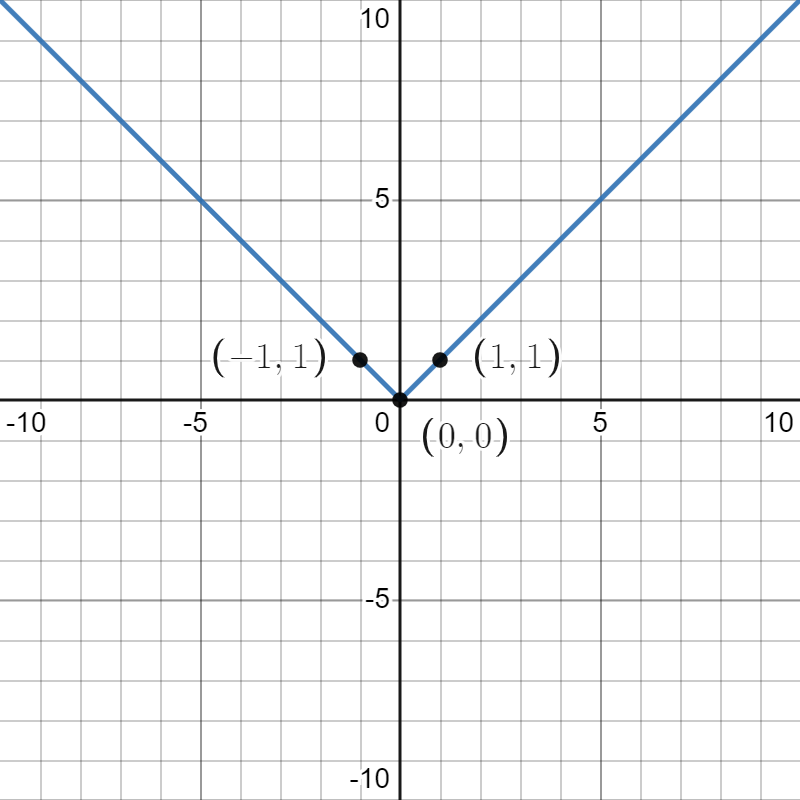
\includegraphics[width=1\linewidth]{images/exgraph1.png}

After horizontally shifting right  by 5 units, our points are $(5, 0)$, $(6, 1)$, and $(4, 1),$ and the graph of $f_1(x) = f_0(x - 5) = |x - 5|$ looks like this:

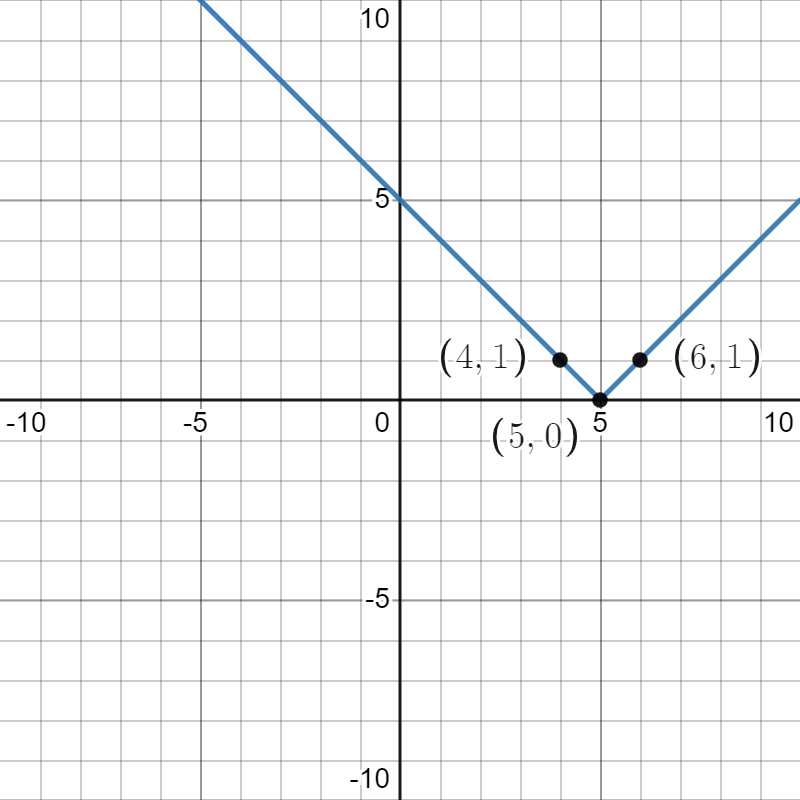
\includegraphics[width=1\linewidth]{images/exgraph2.png}

Compressing horizontally by a factor of 3 gives us $f_2(x) = f_1(3x) = |3x - 5|$, and our points are $\left(\frac{5}{3}, 0\right)$, $(2, 1)$, and $\left(\frac{4}{3}, 1\right)$:

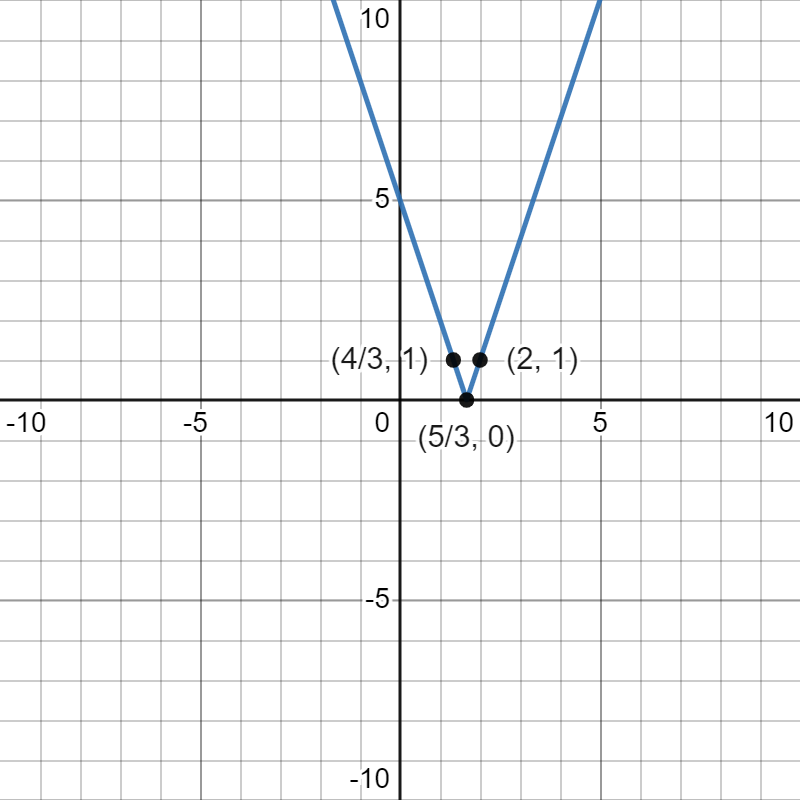
\includegraphics[width=1\linewidth]{images/exgraph3.png}

Vertically compressing by a factor of 2 gives us the points $\left(\frac{5}{3}, 0\right)$, $\left(2, \frac{1}{2}\right)$, and $\left(\frac{4}{3}, \frac{1}{2}\right)$ and the function $f_3(x) = \frac{1}{2}f_2(x) = \frac{1}{2}|3x - 5|$:

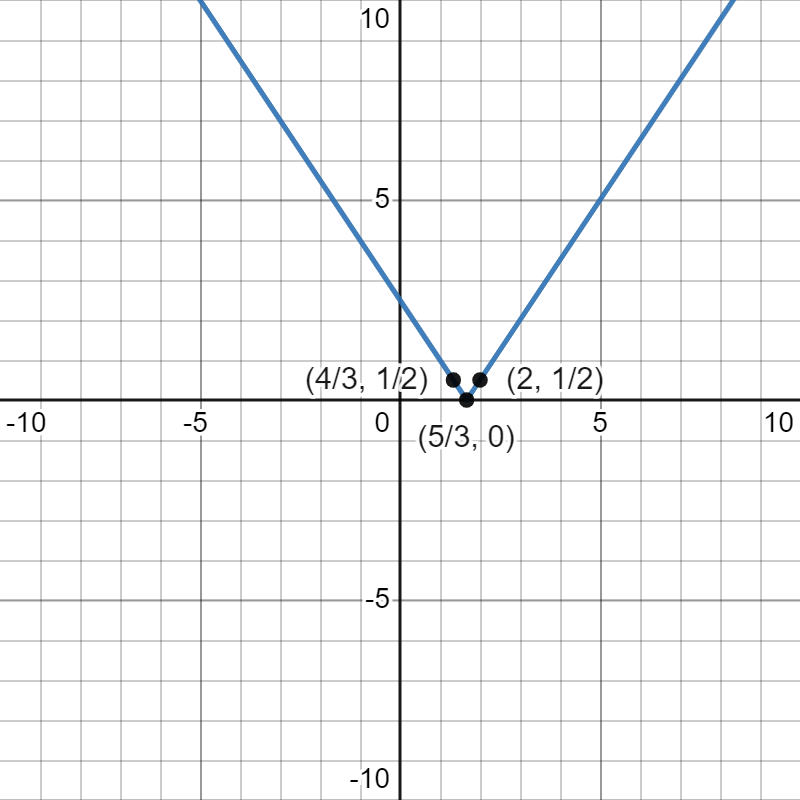
\includegraphics[width=1\linewidth]{images/exgraph4.png}

Reflecting across the $x$-axis gives us the points $\left(\frac{5}{3}, 0\right)$, $\left(2, -\frac{1}{2}\right)$, and $\left(\frac{4}{3}, -\frac{1}{2}\right)$ and the function $f_4(x) = -f_3(x) = -\frac{1}{2}|3x - 5|$:

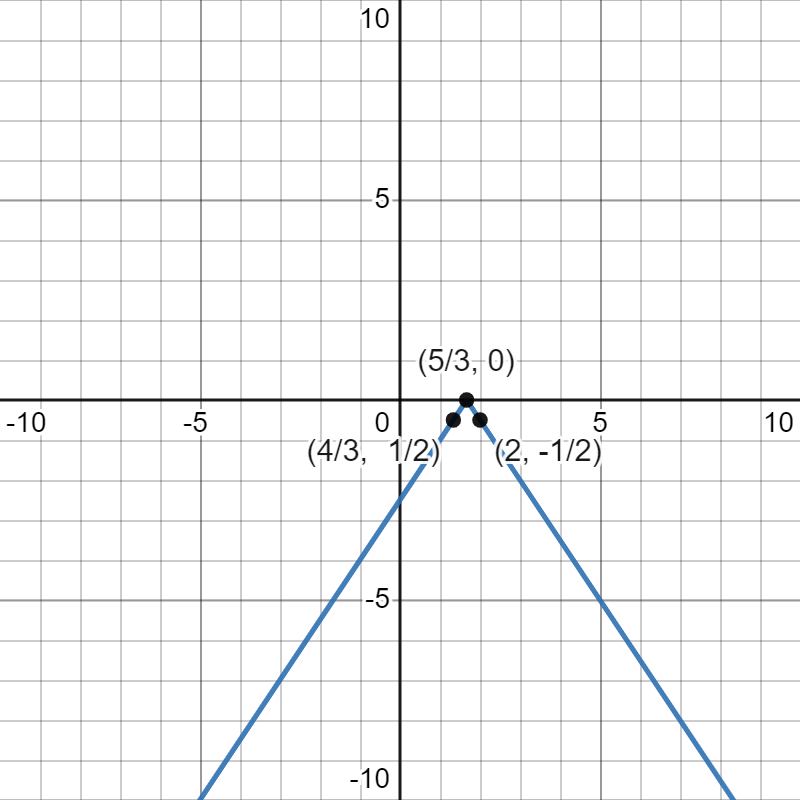
\includegraphics[width=1\linewidth]{images/exgraph5.png}

Finally, vertically shifting up by 1 gives us the points $\left(\frac{5}{3}, 1\right)$, $\left(2, \frac{1}{2}\right)$, and $\left(\frac{4}{3}, \frac{1}{2}\right)$ and the function $f(x) = f_4(x)+ 1 = -\frac{1}{2}|3x - 5| + 1$:

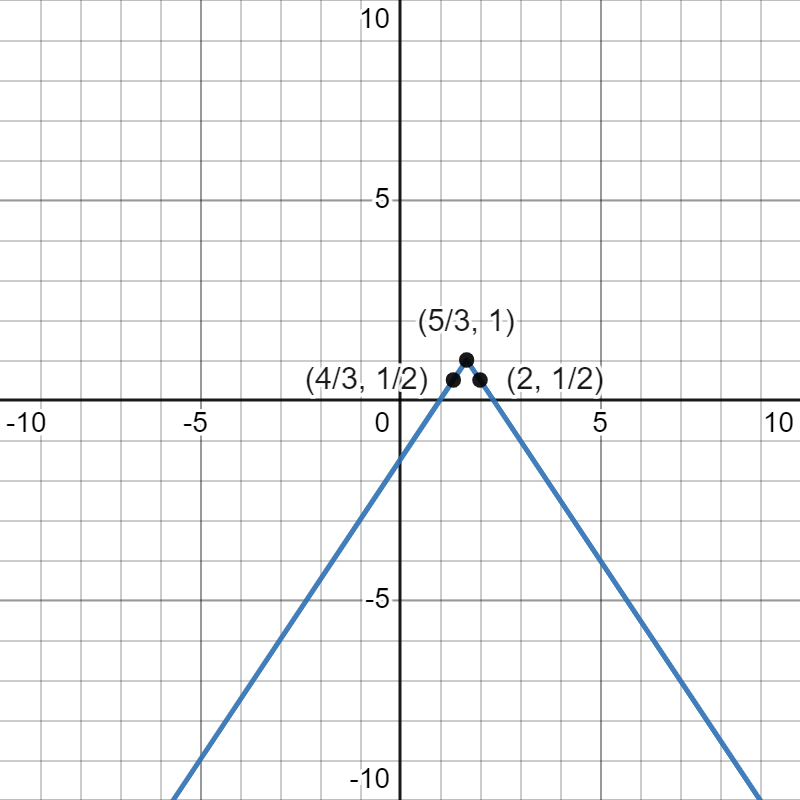
\includegraphics[width=1\linewidth]{images/exgraph6.png}

This last graph is our final result. While graphing each step along the way may seem like an awful lot of work, it is often easier than trying to work with multiple transformations at once in your head. 
\end{explanation}
\end{example}

Below is a link to a Desmos graph containing $af(bx + h) + k$ for a function $f$ where you can adjust the values of $a$, $b$, $h$, and $k$ to see how they affect the graph. 

\begin{center}  
\desmos{wf5aevwjhk}{800}{600}  
\end{center}



%\typeout{************************************************}
%\typeout{Summary}
%\typeout{************************************************}

\begin{summary}\begin{itemize}
\item Multiple transformations can be applied to a parent function.
\item The order in which transformations are applied can change the resulting function.
\item Given a formula of a transformed function, we can infer the order of transformations that produced it, as well as graph the function. 
\end{itemize}\end{summary}




\end{document}
